\hypertarget{FirmaDigital_8cpp}{}\section{Referencia del Archivo Template\+A\+F\+I\+S\+\_\+webservice\+\_\+lib/firma\+\_\+digital/\+Firma\+Digital.cpp}
\label{FirmaDigital_8cpp}\index{Template\+A\+F\+I\+S\+\_\+webservice\+\_\+lib/firma\+\_\+digital/\+Firma\+Digital.\+cpp@{Template\+A\+F\+I\+S\+\_\+webservice\+\_\+lib/firma\+\_\+digital/\+Firma\+Digital.\+cpp}}


Se definen los métodos para generar la clave que será la firma de cada paquete X\+M\+L-\/\+R\+PC.  


{\ttfamily \#include $<$iostream$>$}\newline
{\ttfamily \#include $<$stdio.\+h$>$}\newline
{\ttfamily \#include $<$stdlib.\+h$>$}\newline
{\ttfamily \#include $<$sstream$>$}\newline
{\ttfamily \#include $<$string$>$}\newline
{\ttfamily \#include $<$ctime$>$}\newline
{\ttfamily \#include \char`\"{}md5.\+h\char`\"{}}\newline
Dependencia gráfica adjunta para Firma\+Digital.\+cpp\+:\nopagebreak
\begin{figure}[H]
\begin{center}
\leavevmode
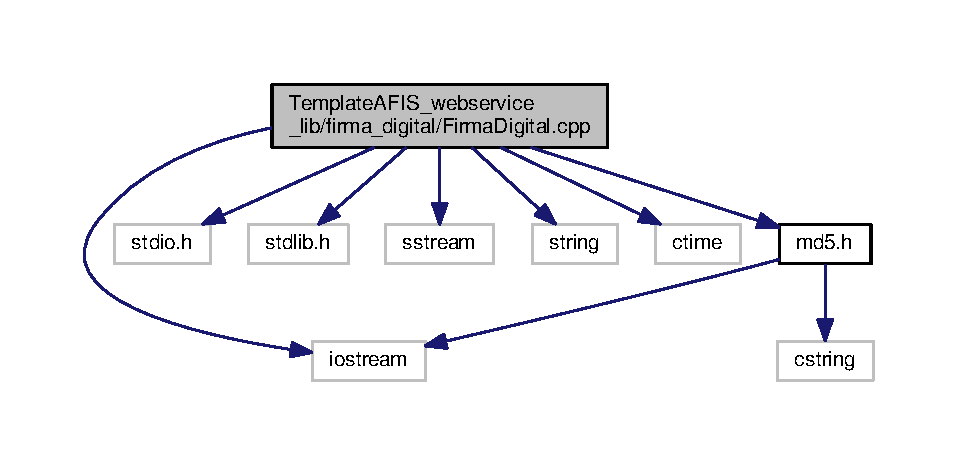
\includegraphics[width=350pt]{FirmaDigital_8cpp__incl}
\end{center}
\end{figure}


\subsection{Descripción detallada}
Se definen los métodos para generar la clave que será la firma de cada paquete X\+M\+L-\/\+R\+PC. 

Comando de compilación\+: g++ \hyperlink{sha512_8cpp}{sha512.\+cpp} firma\+\_\+srcl.\+cpp -\/o firma\+\_\+srcl \&\& ./firma\+\_\+srcl

\begin{DoxyAuthor}{Autor}
Asociación Cooperativa Simón Rodríguez para el Conocimiento Libre. \href{mailto:contacto@simonrodriguez.org.ve}{\tt contacto@simonrodriguez.\+org.\+ve} 
\end{DoxyAuthor}
\begin{DoxyDate}{Fecha}
2014 This file is part of Sistema de Identificación Biométrica para las O\+B\+PP. 
\end{DoxyDate}
